%======================================================================
\NEWSEC
%======================================================================

\subsection{\ssCharmCello}

\begin{frame}[fragile,label=ss-charm-cello] 
% ----------------------------------------------------------------------
\secframetitle{\ssCharmCello}
\begin{itemize}
\item \code{Enzo-P} begins in the \cyancode{mainchare}
\begin{itemize}
\item single chare on root process
\item creates a \redcode{Simulation} chare group
\end{itemize}
\item \redcode{Simulation} stores ``global'' data
\begin{itemize}
\item one \redcode{Simulation} object per physical process
\item creates \bluecode{Block} chare array
\end{itemize}
\item \bluecode{Block}s associated with octree nodes
\begin{itemize}
\item many \bluecode{Block}s per process
\item indexed using bit-coding of location
\end{itemize}
\end{itemize}

\end{frame}

\begin{frame}[fragile] 
% ----------------------------------------------------------------------
\secframetitle{\ssCharmCello}
\begin{center}
\begin{minipage}{1.00in}
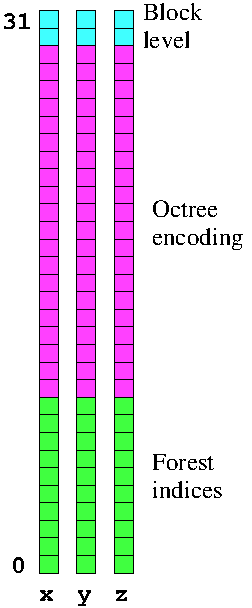
\includegraphics[width=1.0in]{index.pdf}
\end{minipage}
\begin{minipage}{3.25in}
\begin{itemize}
\item User-defined chare array indices supported
\item \cello\ indices for \code{Block} arrays:
\begin{itemize}
\item $3 \times 10 $ bits for \greenit{forest indices} 
\item $3 \times 20 $ bits for the \magentait{octree encoding}
\item $6$ bits for the \cyanit{block level}
\end{itemize}
\item Up to $1024^3$ array of octrees
\item Up to $20$ octree levels
\item $-31 \le$ level $\le 31$
\item Block id's use index: e.g. \bluecode{B100:11\_1:01}
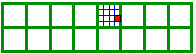
\includegraphics[width=1.2in]{block-index.pdf}
\end{itemize}
\end{minipage}
\end{center}
\end{frame}
%----------------------------------------------------------------------


